\documentclass[letterpaper, 11pt]{article}

\usepackage[total={6.5in, 9in}]{geometry}
\usepackage[utf8]{inputenc}
\usepackage[T1]{fontenc}
% \usepackage{adjustbox}
\usepackage{amsmath}
\usepackage{graphicx}
% \usepackage{amsmath,amssymb,latexsym}
% \usepackage{fullpage}
\usepackage{enumitem}
\usepackage{hyperref}
\usepackage{url}
\usepackage{cite}
\usepackage{indentfirst}
\usepackage[font=footnotesize,labelfont=it]{caption}

\hypersetup{
    colorlinks=true,
    linkcolor=blue,
    filecolor=magenta,      
    urlcolor=cyan,
}

\setlength{\parindent}{0.25in}
\setlength{\parskip}{11pt}

\renewcommand{\labelitemii}{$\circ$}

% \graphicspath{{../}}

\title{\LARGE\bfseries Continuity Report:\\Revisiting Grocery Recognition using TensorFlow}
\author{Samuel C.~Hoffman, Dilip Thiagarajan\\
		\texttt{\{sch235, dt372\}@cornell.edu}}
\date{Last Updated: \today}


\begin{document}

\maketitle

\vspace*{-22pt}

\section{Introduction}

% problem description, background, GroZi project history

The revolution of convolutional neural networks (ConvNets) in the field of machine learning has spawned applications in a wide array of areas. Some accessibility applications have already begun to harness the potential of ConvNets in computer vision for assisting the visually impaired such as Facebook's Automatic Alternative Text tool for narrating images \cite{fair16} However, the underlying technology involved in recognizing grocery items to assist visually impaired shoppers has not advanced much beyond the study by Merler, Galleguillos, and Belongie \cite{merler07}. We aim to revisit this study and apply modern deep convolutional neural networks to solve the problem. We will use the open source library, TensorFlow\footnote{\texttt{\href{https://www.tensorflow.org/}{https://www.tensorflow.org/}}}, to implement the deep learning system \cite{tensorflow15}.

We attempt to solve the problem of recognizing objects in the wild using images of the object taken under ideal conditions to train. This challenge has enumerable applications but in this study, we will look specifically at recognizing grocery products sold in Mattin's, a local caf\'{e} on the Cornell campus in Ithaca. However, the results should be easily transferrable to other areas of application. Ideally, training data and testing data would be obtained from the same distribution, however, in real-world applications, it is often more convenient to obtain training data from the web or dedicated datasets. Ultimately, our goal in this study is to achieve real-time recognition and localization with a camera.

The GroZi project\footnote{\texttt{\href{http://grozi.calit2.net/}{http://grozi.calit2.net/}}}, from which the original study came, encompasses many applications surrounding this core recognition problem. However, the implementation still relies on color histogram matching, SIFT matching, and boosted Haar-like features and the results left room for improvement.

For further background, please read our original proposal.\footnote{\texttt{\href{https://github.com/dthiagarajan/grozi_tf/blob/master/proposal/Proposal.pdf}{https://github.com/dthiagarajan/grozi\_tf/blob/master/proposal/Proposal.pdf}}}

\section{Approach}

% methods you attempted, motivation for chosen algorithms

\noindent In this section, we will explain the methods we attempted and motivations for the algorithms we chose.

\subsection{TensorFlow}

We settled on using TensorFlow as the main library for implementing our deep learning network. In summary, our reasons for choosing TensorFlow are as follows. While it does not offer significant speed or functionality improvements over other popular libraries, TensorFlow does allow for development entirely in Python. This means we can implement networks quickly without learning the semantics of a new language while allowing for easy integration in any workflow (e.g. processing with NumPy or Scikit-learn). Moreover, Tensorflow is designed to work seamlessly with multiple GPUs and speed is on par with other popular libraries. \cite{lipton15}

\subsection{Data Collection}

In this study, we used the original GroZi-120 dataset for training and testing. The goal of this study is ultimately to recognize groceries at Mattin's, however we haven't collected images of those products yet. We decided our system should be easily applicable to any product set, and thus there was no reason to test at Mattin's until the system worked well enough on the GroZi dataset first.

As we will discuss later, the GroZi-120 dataset was not compiled with deep learning in mind and many products have fewer than 10 images total. After running a few algorithms on the data as is, we attempted to augment the dataset with more canonical images per class. However, this proved difficult since there are only a couple angles at which the products are shot. We briefly explored the idea of collecting data for each item in a controlled environment ourselves, but that process would not scale well and we lacked the resources and time \cite{DBLP:conf/aaai/SappSN08} Some manufacturers have also updated the packaging of products in the dataset and so the exact product is no longer produced.

\subsection{Deep Learning Models}

\noindent Implementation details for all algorithms used can be found on our public GitHub repository.\footnote{\texttt{\href{https://github.com/dthiagarajan/grozi_tf/}{https://github.com/dthiagarajan/grozi\_tf/}}}

\subsubsection{CIFAR-10 Network}

To get a sense of the problem and familiarize ourselves with TensorFlow, we started off with a simple model adapted from a network designed to perform on the CIFAR-10 dataset. The model was not pre-trained on any dataset and used only the data from GroZi-120. Furthermore, we narrowed the classification task to two classes: images of Tide laundry detergent or images of a different product. The images in the second class were drawn uniformly at random from each of the 119 other classes.

In the training phase of this network, we employed basic data augmentation such as random cropping and scaling. Even with this, the dataset was still small and we opted to mix in some of the cropped video stills from the \textit{``in situ''} set. The rest were reserved for testing and validation. Since doing this shrunk the testing set, we decided to employ data augmentation on that set as well.

The results will be discussed in the next section but in summary, the network overfit the data significantly and ROC curves showed poor performance.

We also attempted to adapt an AlexNet architecture with the same parameters as above with similar results.

\subsubsection{Fine-tuning with Inception-v3}

In an attempt to improve the performance with such a small training dataset, we decided to fine-tune Google's Inception network which was trained on the ImageNet dataset. Transfer learning has been shown to improve recognition especially on small datasets \cite{donahue13}. We also decided to look at all 120 classes and plot ROC curves in a one-vs-rest fashion.

The results were disappointing again and we realized we needed a new strategy. Adding complexity to the model increased overfitting but less complex models were not accurate enough.

\subsubsection{Update GroZi Dataset}

The first idea we had was to improve the GroZi dataset, adding new images for each category and updating discontinued products. The plan was to make the dataset more viable for deep learning with hundreds of images per class.

As noted earlier, however, it was difficult to obtain enough data without purchasing the items and capturing images ourselves and therefore this method would not scale well to new items.

\subsubsection{Recognition with Few Training Images}

At this point, we returned to the original problem of recognizing products from just a few \textit{``in vitro''} images. First, we tried increasing the pre-processing and live data augmentation to mimic new data. This involved augmenting training data with randomized backgrounds and pose variations in addition to generic cropping, rotation, scaling, and photometric transformations \cite{DBLP:journals/corr/MasiTLHM16,DBLP:conf/avss/McLaughlinRM15,DBLP:journals/corr/ChatfieldSVZ14}. We also investigated leveraging features at different scales (and thus more data per image) like more traditional computer vision techniques \cite{DBLP:conf/dicta/ZhangWHL09}.

We also investigated a promising study which involved pre-training on rotated objects to learn novel poses with only a few training images \cite{DBLP:journals/corr/HeldTS15}. We chose this strategy, along with the data augmentation procedures mentioned, with which to proceed.

\section{Results}

% experimental performance

\subsection{CIFAR-10 Network}

Our first experiment which trained on the adapted CIFAR network to recognize binary classes (Tide laundry detergent or not) had poor performance. While it achieved an accuracy of around 96\% even with overfitting, this was mostly because the testing images so closely resembled the training images. The ROC curve reveals deeper problems and that the confidence for each image was low.

\begin{figure}[!ht]
	\centering
	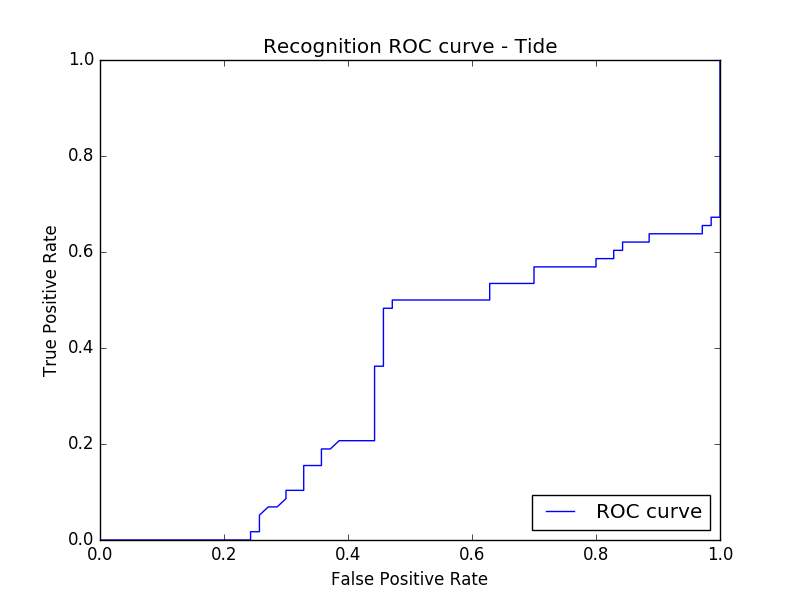
\includegraphics[height=3in]{../tide/ROC_tide_cifar10network}
	\caption{Tide vs not-Tide from CIFAR-10 network with distorted training and testing data}
\end{figure}

\subsection{Fine-tuning with Inception-v3}

From the next figure, we can see that the fine-tuning did not significantly improve the ROC curves for the binary classification case.

\begin{figure}[!ht]
	\centering
	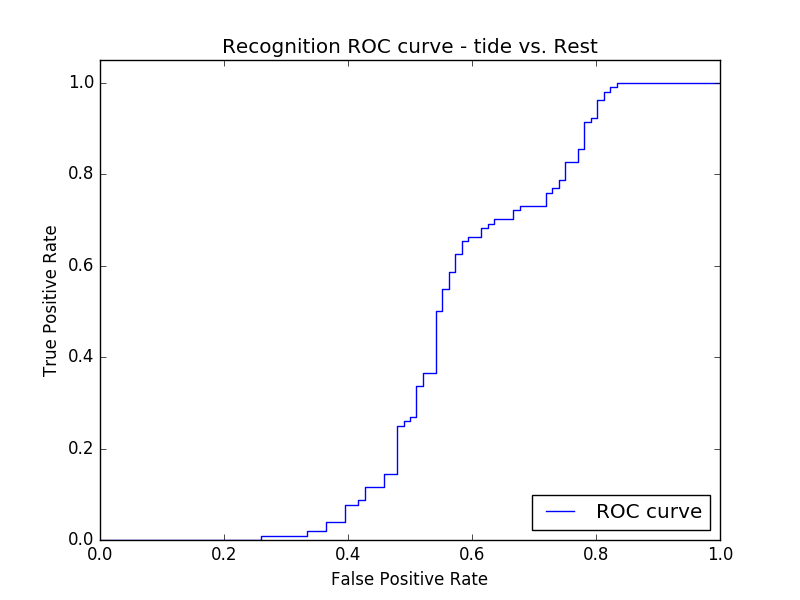
\includegraphics[height=3in]{../roc_curves/roc_curve_tide_vs_rest}
	\caption{Tide vs not-Tide from fine-tuned Inception network with distorted training and testing data}
\end{figure}

After generalizing to all 120 classes, the curves still demonstrate underwhelming performance. Most looked like figure 3 below.\footnote{For more ROC curves, see \texttt{\href{https://github.com/dthiagarajan/grozi_tf/blob/master/roc_curves}{https://github.com/dthiagarajan/grozi\_tf/blob/master/roc\_curves}}}

\begin{figure}[!ht]
	\centering
	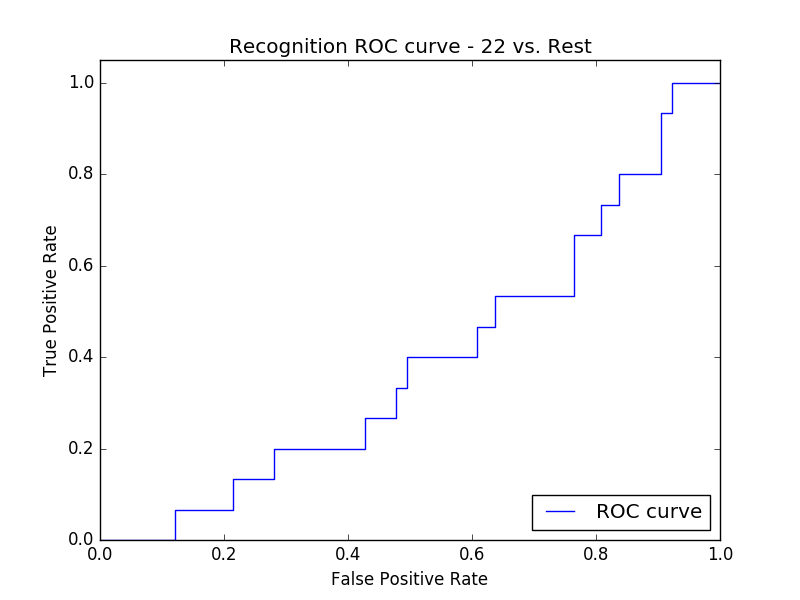
\includegraphics[height=3in]{../roc_curves/roc_curve_22_vs_rest}
	\caption{Dentyne Ice gum vs all other products from fine-tuned Inception network, a representative example of the ROC curves obtained from this network}
\end{figure}

\section{Discussion}

% what worked, what didn’t, recommendations/advice for continued research

After experimenting with simple networks such as the CIFAR network and retraining the Inception network, we set about writing our own networks to test. TensorFlow makes some tasks extremely easy and others unnecessarily complex. In addition to making development slow, it made the networks difficult to understand as a reader and so we turned to a higher-level API to simplify the structure of our code. There were a few options since TensorFlow was open-source and fairly new and at the time of our study, there was no clear popular favorite. We chose TFLearn which seemed to be very functional and extensible.\footnote{\texttt{\href{http://tflearn.org/}{http://tflearn.org/}}}

This ended up causing a few problems when we tried to use our networks for experimentation. While TFLearn allows for the restoration of weights and variables, it uses a format which requires the training to be done using TFLearn also. Since training on large datasets such as ImageNet requires many GPUs or a lot of time, we were limited to using networks for which there were pre-trained weights, which at the time was only VGG-16. This in turn caused problems since VGG-16 would use more memory than was available on our AWS instance and would crash.

In the future, we would recommend writing functions to automate common TensorFlow tasks without using a third-party API to make development easier or using a more mature API. Although we did find a tool for converting pre-trained Caffe models to TensorFlow, we were unable to test this tool ourselves.\footnote{\texttt{\href{https://github.com/ethereon/caffe-tensorflow}{https://github.com/ethereon/caffe-tensorflow}}} Furthermore, while Amazon Web Services does make training with a GPU easy, the instances are limited to 4GB of video memory and do not always offer large speed improvements.

For continued research, we recommend starting by looking at the Held study \cite{DBLP:journals/corr/HeldTS15} and researching other attempts at deep learning with small training data sets. The field of unsupervised learning is also growing rapidly and so more research in that direction seems promising and might yield some insights for small datasets.

\newpage
\nocite{DBLP:journals/corr/GeorgeMSFM15}
\bibliographystyle{abbrv}
\bibliography{refs}

\newpage
\appendix
\section{Appendix}

% code listing and/or pointers to code repo

Project repository:

\begin{center}
\texttt{\href{https://github.com/dthiagarajan/grozi_tf/}{https://github.com/dthiagarajan/grozi\_tf/}}
\end{center}

GroZi-120 dataset:
\begin{center}
\texttt{\href{http://grozi.calit2.net/grozi.html}{http://grozi.calit2.net/grozi.html}}
\end{center}

\end{document}